% Created 2022-10-11 Tue 21:57
% Intended LaTeX compiler: pdflatex
\documentclass[11pt]{article}
\usepackage[utf8]{inputenc}
\usepackage[T1]{fontenc}
\usepackage{graphicx}
\usepackage{longtable}
\usepackage{wrapfig}
\usepackage{rotating}
\usepackage[normalem]{ulem}
\usepackage{amsmath}
\usepackage{amssymb}
\usepackage{capt-of}
\usepackage{hyperref}
\usepackage{float}
\author{Mohammad Hasani, MD}
\date{\today}
\title{Childhood Obesity and Testicular Volume}
\hypersetup{
 pdfauthor={Mohammad Hasani, MD},
 pdftitle={Childhood Obesity and Testicular Volume},
 pdfkeywords={},
 pdfsubject={},
 pdfcreator={Emacs 29.0.50 (Org mode 9.6)}, 
 pdflang={English}}
\makeatletter
\newcommand{\citeprocitem}[2]{\hyper@linkstart{cite}{citeproc_bib_item_#1}#2\hyper@linkend}
\makeatother

\usepackage[notquote]{hanging}
\begin{document}

\maketitle
\setcounter{secnumdepth}{0}

\begin{center}
\textbf{Supervisor}
\end{center}

Sosan Jafarian, Pediatrician, Department of Pediatrics, Faculty of Medicine, School of Medicine, Shahroud Azad University, Semnan, Iran

\begin{center}
\textbf{Mentors}
\end{center}

\begin{enumerate}
\item Abbas Tavakolian Arjmand, Internist, Endocrinologist, Department of Internal Medicine, Faculty of Medicine, School of Medicine, Shahroud Azad University, Semnan, Iran
\item Ahmad Khosravi, Epidemiologist, Department of Social Medicine, Faculty of Medicine, Shahroud University of Medical Sciences, Semnan, Iran
\end{enumerate}

\break

\tableofcontents

\break

\section{Introduction}
\label{sec:orgf542b39}
Infertility has risen dramatically, and sperm count has declined 50-60\% in the past 40 years worldwide\textsuperscript{\citeprocitem{1}{1(p654)}}.
Beyond the fertility concerns, studies suggested reduced sperm count predicts increased all-cause mortality and morbidity\textsuperscript{\citeprocitem{2}{2(pp560-561)}}.
Meanwhile, we are in a pandemic of obesity due to metabolic syndrome\textsuperscript{\citeprocitem{3}{3}} and studies at population level and infertile couples shows that the obesity is associated with reduced male fertility\textsuperscript{\citeprocitem{4}{4(p902)}}.

Testicular volume is an \textbf{easy clinical marker} which generally is supposed to correlate well with semen quality and fertility\textsuperscript{\citeprocitem{5}{5(p416)}}.

Based on these findings, if there be a relationship between obesity and testicular volume, it would be a good practice for pediatricians as a screening to begin routinely assessing testicular volume at all visits as is now done with height and weight, to \textbf{\textbf{identify early deflection of the testicular growth curve}}.

\section{Review of The Literature}
\label{sec:org984cc5a}
A literature search with the string ``obes* AND ((small* OR (low volume)) AND (testis OR testes))'' on \textit{18 Aug 2022} in the Google Scholar, PubMed, and Cochrane library databases was performed which didn't result in any study with exact aim\footnote{Also a literature search through SID, Civilica, and IranDoc with the persian translation of the topic performed which didn't result in any enhancement.}.
For further investigation search with the same string in the Google search engine on \textit{18 Aug 2022} led to a conference news article at Medscape mentioning a session from ENDO 2022 conference at \textit{12/06/22 Sun 11:00}.
Full text of all documents reviewed throughly and carefully on \textit{19 Aug 2022} to provide a research foundation in the topic.

According to a study by Cannarella et al. on 264 male children and adolescents, testicular volume was lower and start of puberty was delayed in those with overweight or obesity compared with normal weight\textsuperscript{\citeprocitem{6}{6}}.
Recent Italian studies shown 14-23\% of young men aged 18-19 had testicular hypotrophy without a clear reason\textsuperscript{\citeprocitem{6}{6}}!
Obesity has been proposed to affect male fertility both directly and indirectly, by inducing alterations in sleep and sexual behavior, hormonal profile, scrotal temperature and semen parameters\textsuperscript{\citeprocitem{4}{4(pp899-901)},\citeprocitem{7}{7(pp157-158)}}.
Obese males have higher circulating estrogen level as a result of aromatization in the fat tissue which can be an important mechanism for the hypoandrogenemia and altered sperm parameters\textsuperscript{\citeprocitem{4}{4(p902)},\citeprocitem{7}{7(p158)}}.

\section{Research Gaps}
\label{sec:org32ac5d0}
As the literature review revealed, there is little established studies around the relationship of childhood obesity and testicular volume.
Moreover, further longitudinal studies are needed to establish a possible cause-and-effect relationship\textsuperscript{\citeprocitem{6}{6}}.
Although there are evidences that imply weight reduction can correct hormonal imbalance in obese patients, but these data need to be complemented by studies showing the effect of weight loss on sperm parameters and fertility\textsuperscript{\citeprocitem{4}{4},\citeprocitem{8}{8}}.

\section{Research Design and Methods}
\label{sec:org54930dd}
Among various types of correlational research methods we prefered to lead a cross-sectional study as it is the simplest, plausible, and fastest method to reveal a possible relationship between childhood obesity and testicular volume.
However a cross-sectional study is unable to reveal a cause-and-effect relationship, but it provides initial indication and additional support for future studies.

Target research population are male children aged 8-11 in Shahroud, Semnan, Iran;
Elementary schools in the city selected as the sampling frame.
To collect sample, we will
\textbf{1.} Select a convenient school randomly;
\textbf{2.} Schedule an interview with the school principals to
\textbf{3.} Schedule an interview with parents to explaining the research, encouraging them to participate in the research, and distributing the informed consent form between them;
\textbf{4.} As long as necessary, we will back to \textbf{step 1} to collect enough sample.
Due to lack of enough data, it is not possible to state a reasonable and pragmatic sample size prediction.
To overcome this issue, we will direct a pilot research to obtain enough data and predict the sample size.

\subsection{Sample Inclusion Criteria}
\label{sec:orgc884046}
Participants must have willingness to participate in the study as the only inclusion criteria.

\subsection{Sample Exclusion Criteria}
\label{sec:org926d2b0}
As the study isn't longitudinal, there is no applicable exclusion criteria.

\subsection{Data Collection}
\label{sec:orgbb9963b}
\begin{enumerate}
\item Each participant will be invited to a free-charged pediatrician interview at the polyclinic of Khatam-al-Anbia hospital in Shahroud;
\item A skilled research executive will take relevant history, including:
\begin{itemize}
\item Identifying information;
\item Contact information;
\item Age;
\item School;
\end{itemize}
\item A skilled research executive will perform relevant physical examination, including:
\begin{itemize}
\item Height;
\item Weight using a standard and calibrated medical office weight scale;
\item Waist circumference using superior border of Iliac crest as the landmark and placing measuring tape parallel to the floor around the abdomen\textsuperscript{\citeprocitem{9}{9(fig3)}}.;
\item Testicular volume using a standard Prader's orchidometer;
\end{itemize}
\item Obtained data will be recorded.
\end{enumerate}

\subsection{Data Analysis}
\label{sec:org99eb8be}
Data transfomration methods will be used as needed; \(\alpha\)=0.05;

\renewcommand{\arraystretch}{1.5}

\begin{sidewaystable}[htbp]
\centering
\begin{tabular}{l|l|l|l|p{6cm}}
Name & Role & Type & Unit (SI) & Measurement Method\\
\hline
BMI & Independent & Continuous quantitative & kg/m\textsuperscript{2} & N/A\\
Waist circumference & Independent & Continuous quantitative & cm & Using superior border of Iliac crest as the landmark and placing measuring tape parallel to the floor around the abdomen\textsuperscript{\citeprocitem{9}{9(fig3)}}.\\
Testicular volume & Dependent & Discrete quantitative & mL & Using a Prader's orchidometer.\\
Age & Confounding & Continuous quantitative & year & N/A\\
School & Contextual & Nominal & N/A & N/A\\
\end{tabular}
\caption{Variables}

\end{sidewaystable}

\begin{figure}[H]

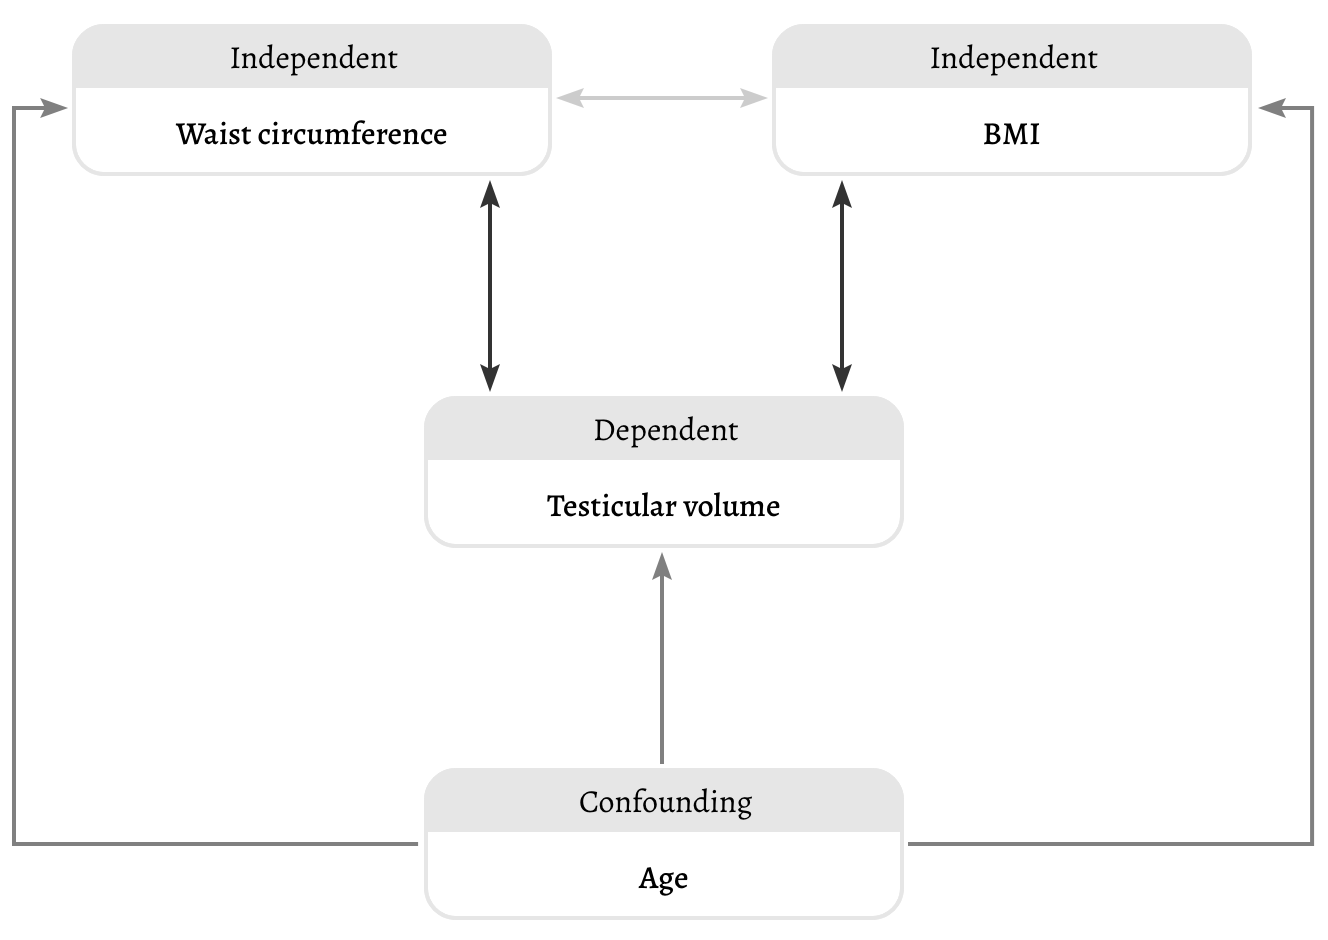
\includegraphics[width=\linewidth]{./images/conceptual-framework.png}
\caption{conceptual framework}
\end{figure}

\section{Research Objectives}
\label{sec:orgf904d22}
The general aim of this study is to determine possible relationship of childhood obesity and testicular volume.

\noindent
Speaking specifically:
\begin{itemize}
\item Measure testicular volume in obese group.
\item Measure testicular volume in overweight group.
\item Measure testicular volume in normal weight group.
\item Compare testicular volume in obese, overweight, and normal weight groups.
\end{itemize}

\section{Research Questions}
\label{sec:orgf908f16}
\begin{itemize}
\item How much is testicular volume in obese group?
\item How much is testicular volume in overweight group?
\item How much is testicular volume in normal weight group?
\item What is difference of testicular volume in obese, overweight, and normal weight groups?
\end{itemize}

\section{Research Hypothesis}
\label{sec:org831c898}
\textbf{H0}: There is no difference between testicular volume of normal weight, overweight, and obese children.

\noindent
\textbf{H1}: There is a difference between testicular volume of normal weight, overweight, and obese children.

\section{Research Importance/Innovation?}
\label{sec:orgedd3502}
This is one of the first coherent cross-sectional study to determine possible relationship of childhood obesity and testicular volume in Iran.

\section{Beneficiaries}
\label{sec:org0f84feb}
\begin{itemize}
\item Physicians;
\item General population;
\item Researchers in other disciplines;
\item Academic organisations;
\item Ministry of Health and Medical Education of Iran;
\end{itemize}

\section{Conflicts of Interest}
\label{sec:org9f14951}
No conflict of interest was declared.

\section{Keywords}
\label{sec:org6bc8cb2}
Pediatric, child health, children's health, child well being,
obesity, overweight,
male,
infertility, sub-fertility, sterility,
testicular volume.

\section{Bibliography}
\label{sec:org04f8734}
\hypertarget{citeproc_bib_item_1}{1. Levine H, Jørgensen N, Martino-Andrade A, et al. Temporal trends in sperm count: A systematic review and meta-regression analysis. \textit{Human reproduction update}. 2017;23(6):646-659. doi:\href{https://doi.org/10.1093/humupd/dmx022}{10.1093/humupd/dmx022}}

\hypertarget{citeproc_bib_item_2}{2. Jensen TK, Jacobsen R, Christensen K, Nielsen NC, Bostofte E. Good Semen Quality and Life Expectancy: A Cohort Study of 43,277 Men. \textit{American journal of epidemiology}. 2009;170(5):559-565. doi:\href{https://doi.org/10.1093/aje/kwp168}{10.1093/aje/kwp168}}

\hypertarget{citeproc_bib_item_3}{3. Grundy SM. Metabolic Syndrome Pandemic. \textit{Arteriosclerosis, thrombosis, and vascular biology}. 2008;28(4):629-636. doi:\href{https://doi.org/10.1161/ATVBAHA.107.151092}{10.1161/ATVBAHA.107.151092}}

\hypertarget{citeproc_bib_item_4}{4. Hammoud AO, Gibson M, Peterson CM, Meikle AW, Carrell DT. Impact of male obesity on infertility: A critical review of the current literature. \textit{Fertility and sterility}. 2008;90(4):897-904. doi:\href{https://doi.org/10.1016/j.fertnstert.2008.08.026}{10.1016/j.fertnstert.2008.08.026}}

\hypertarget{citeproc_bib_item_5}{5. Takihara H, Cosentino MJ, Sakatoku J, Cockett ATK. Significance of Testicular Size Measurement in Andrology: II. Correlation of Testicular Size with Testicular Function. \textit{The journal of urology}. 1987;137(3):416-419. doi:\href{https://doi.org/10.1016/S0022-5347(17)44053-5}{10.1016/S0022-5347(17)44053-5}}

\hypertarget{citeproc_bib_item_6}{6. Obesity Linked to Smaller Testes and Possible Infertility. In: \textit{Medscape}. Accessed August 19, 2022. \url{https://www.medscape.com/viewarticle/976289}}

\hypertarget{citeproc_bib_item_7}{7. Du Plessis SS, Cabler S, McAlister DA, Sabanegh E, Agarwal A. The effect of obesity on sperm disorders and male infertility. \textit{Nat rev urol}. 2010;7(3, 3):153-161. doi:\href{https://doi.org/10.1038/nrurol.2010.6}{10.1038/nrurol.2010.6}}

\hypertarget{citeproc_bib_item_8}{8. Mongioì LM, Cimino L, Condorelli RA, et al. Effectiveness of a Very Low Calorie Ketogenic Diet on Testicular Function in Overweight/Obese Men. \textit{Nutrients}. 2020;12(10):2967. doi:\href{https://doi.org/10.3390/nu12102967}{10.3390/nu12102967}}

\hypertarget{citeproc_bib_item_9}{9. National Heart L, North American Association for the Study of Obesity. \textit{The Practical Guide Identification, Evaluation, and Treatment of Overweight and Obesity in Adults}. National Heart, Lung, and Blood Institute; 2000.}
\end{document}
